% !TEX root = ../main.tex
\section{Find the Domain of a Function}
Find the domain of the following functions.

\pairofprobsans%
{$\displaystyle f\left(x\right)=x+4$}{$\displaystyle \left(-\infty, +\infty\right)$}
{$\displaystyle f\left(x\right)=x^2+4x + 5$}{$\displaystyle \left(-\infty, +\infty\right) $}

\pairofprobsans%
{$\displaystyle f\left(x\right)=4$}{$\displaystyle \left(-\infty, +\infty\right)$}
{$\displaystyle f\left(x\right)=\frac{1}{4}$}{$\displaystyle \left(-\infty, +\infty\right)$}

\pairofprobsans%
{$\displaystyle f\left(x\right)=-\sqrt{3}$}{$\displaystyle \left(-\infty, +\infty\right)$}
{$\displaystyle f\left(x\right)=0$}{$\displaystyle \left(-\infty, +\infty\right)$}

\pairofprobsans%
{$\displaystyle f\left(x\right)=x^3 - 5$}{$\displaystyle \left(-\infty, +\infty\right)$}
{$\displaystyle f\left(x\right)=\frac{2}{x+3}$}{$\displaystyle \left(-\infty, -3\right) \cup \left(-3, +\infty\right)$}

\pairofprobsans%
{$\displaystyle f\left(x\right)=\frac{2}{x^2+3}$}{$\displaystyle \left(-\infty, +\infty\right)$}
{$\displaystyle f\left(x\right)=\sqrt{x+3}$}{$\displaystyle \left[-3, +\infty\right)$}

\newpage

\pairofprobsans%
{$\displaystyle f\left(x\right)=\sqrt{x^2+3}$}{$\displaystyle \left(-\infty, +\infty\right)$}
{$\displaystyle f\left(x\right)=\sqrt{x^2+2x-8}$}{$\displaystyle \left(-\infty, -4\right] \cup \left[2, +\infty\right)$}

\pairofprobsans%
{$\displaystyle f\left(x\right)=\log{(x+3)}$}{$\displaystyle \left(-3, +\infty\right)$}
{$\displaystyle f\left(x\right)=\log{\left(x^2+3\right)}$}{$\displaystyle \left(-\infty, +\infty\right)$}

\pairofprobsans%
{$f\left(x\right)=\log{(x^2+2x}$$-8)$}{$\displaystyle \left(-\infty, -4\right) \cup \left(2, +\infty\right)$}
{$\displaystyle f\left(x\right)=2^{x+3}$}{$\displaystyle \left(-\infty, +\infty\right)$}

\pairofprobsans%
{$\displaystyle f\left(x\right)=\frac{\sqrt{x + 3}}{x-2}$}{$\displaystyle \left[-3, 2\right) \cup \left(2, +\infty\right)$}
{$\displaystyle f\left(x\right)=\frac{x + 3}{\log{(x-2)}}$}{$\displaystyle \left(2, 3\right) \cup \left(3, +\infty\right)$}

\problemans%
{$\displaystyle f\left(x\right)=\frac{\sqrt{x + 3}}{x^2-16}$}{$\displaystyle \left[-3, 4\right) \cup \left(4, +\infty\right)$}

%%%% GUIDES
\qrfigure{chapter1/qr/Finding-Domain.png}{Scan for guides}


%----------------------------
%\makenewpage. % Adding line will make hyperref add an extra blank page
\section{Graphs of Functions}

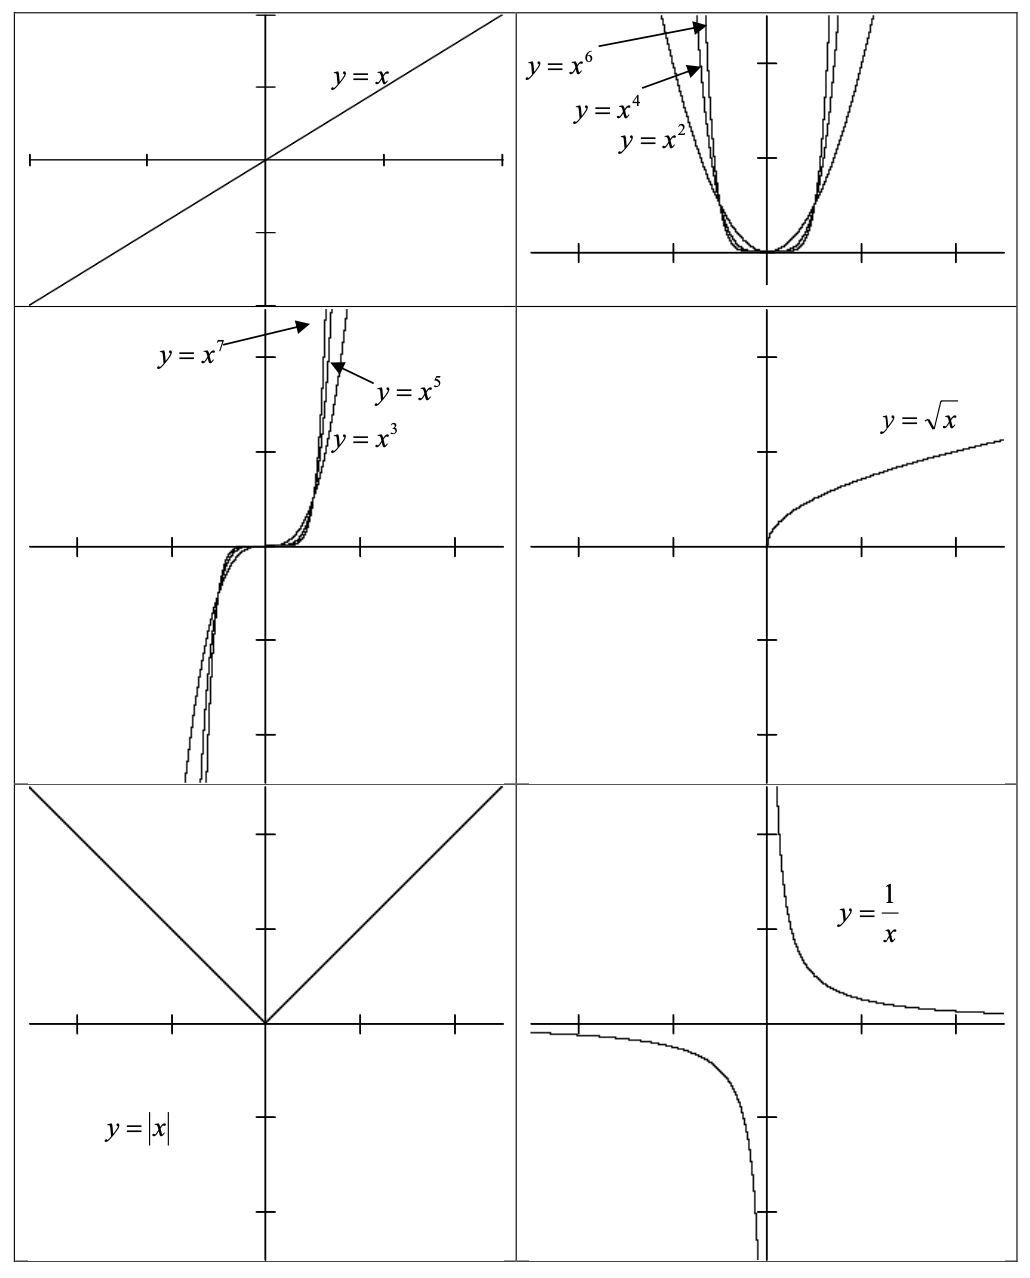
\includegraphics[width=0.7\linewidth]{chapter1/function1}\\
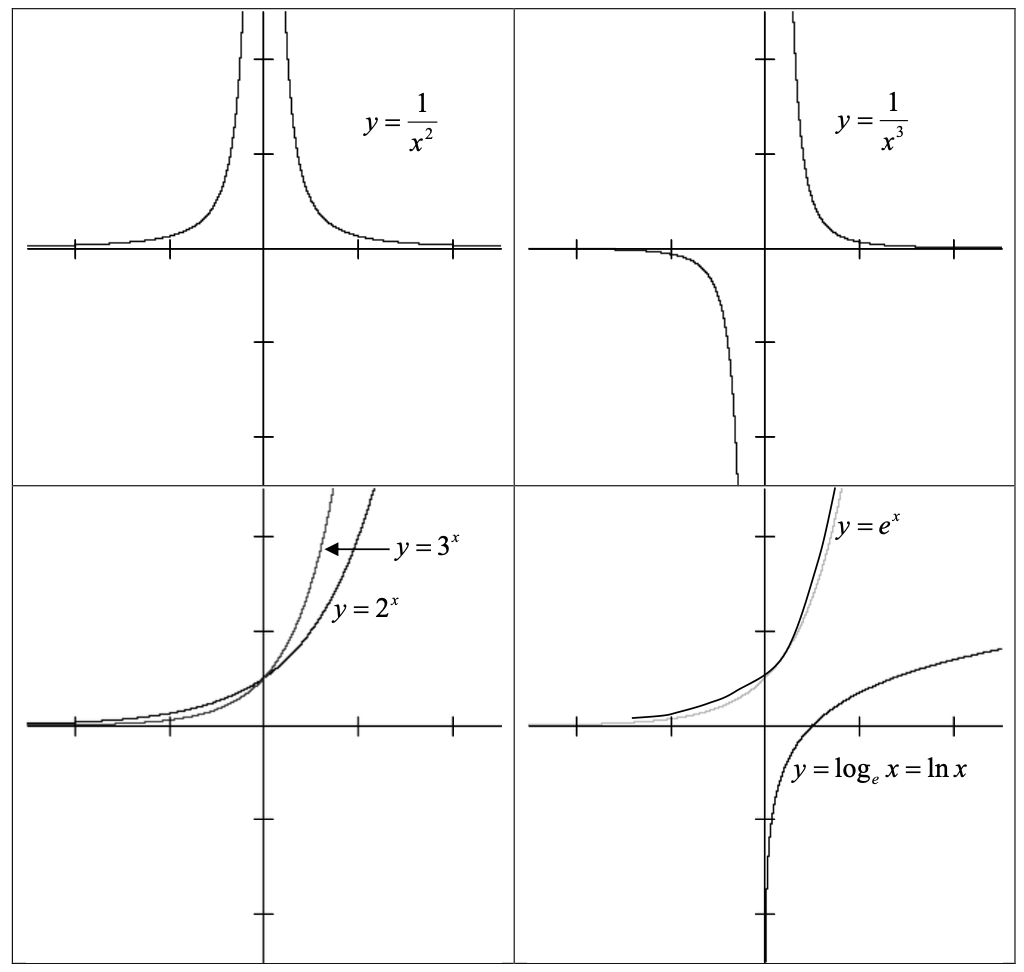
\includegraphics[width=0.7\linewidth]{chapter1/function2}


